\begin{minipage}{0.75\linewidth}
\begin{figure}[h]
    \centering
    \begin{adjustbox}{max width=1.0\linewidth, keepaspectratio}
        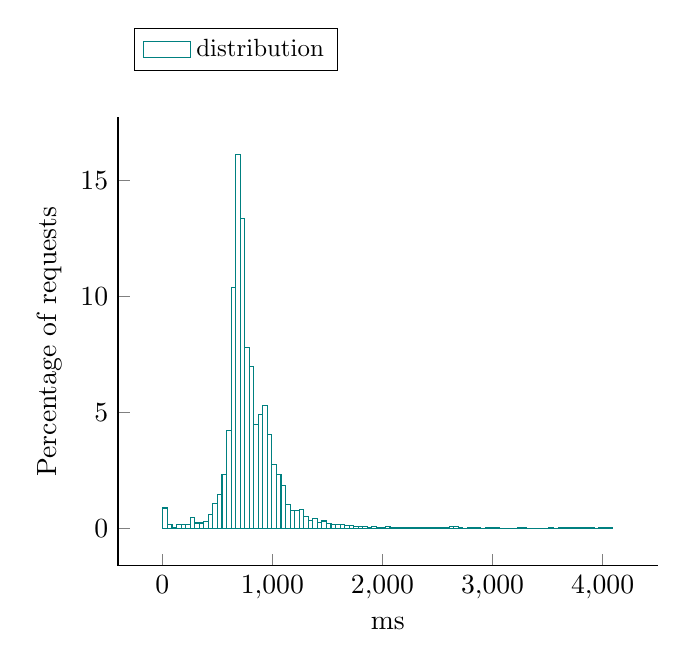
\begin{tikzpicture}
            \begin{axis}[ylabel = Percentage of requests, 
xlabel = ms, 
legend style = {nodes={scale=0.9, transform shape}, at={(0.03,1.2)}, anchor=north west, draw=black, fill=white, align=left, legend columns=3},
area style, mark size = 0pt,
 cycle list name = exotic,
  axis lines* = left]
		\addplot +[ybar interval] coordinates {
			 (6, 0.875547)
			 (47.26, 0.177194)
			 (88.52, 0.0521159)
			 (129.78, 0.177194)
			 (171.04, 0.145925)
			 (212.3, 0.166771)
			 (253.56, 0.479466)
			 (294.82, 0.22931)
			 (336.08, 0.22931)
			 (377.34, 0.281426)
			 (418.6, 0.583698)
			 (459.86, 1.06316)
			 (501.12, 1.46967)
			 (542.38, 2.31395)
			 (583.64, 4.21097)
			 (624.9, 10.3606)
			 (666.16, 16.1038)
			 (707.42, 13.3521)
			 (748.68, 7.78612)
			 (789.94, 6.98353)
			 (831.2, 4.46112)
			 (872.46, 4.88847)
			 (913.72, 5.27413)
			 (954.98, 4.03377)
			 (996.24, 2.76214)
			 (1037.5, 2.30352)
			 (1078.76, 1.83448)
			 (1120.02, 1.01105)
			 (1161.28, 0.771315)
			 (1202.54, 0.750469)
			 (1243.8, 0.802585)
			 (1285.06, 0.500313)
			 (1326.32, 0.343965)
			 (1367.58, 0.416927)
			 (1408.84, 0.250156)
			 (1450.1, 0.312695)
			 (1491.36, 0.19804)
			 (1532.62, 0.156348)
			 (1573.88, 0.145925)
			 (1615.14, 0.156348)
			 (1656.4, 0.114655)
			 (1697.66, 0.114655)
			 (1738.92, 0.0625391)
			 (1780.18, 0.0833854)
			 (1821.44, 0.0833854)
			 (1862.7, 0.0521159)
			 (1903.96, 0.0625391)
			 (1945.22, 0.0312695)
			 (1986.48, 0.0521159)
			 (2027.74, 0.0625391)
			 (2069, 0.0521159)
			 (2110.26, 0.0521159)
			 (2151.52, 0.0312695)
			 (2192.78, 0.0208464)
			 (2234.04, 0.0416927)
			 (2275.3, 0.0208464)
			 (2316.56, 0.0208464)
			 (2357.82, 0.0208464)
			 (2399.08, 0.0416927)
			 (2440.34, 0.0208464)
			 (2481.6, 0.0312695)
			 (2522.86, 0.0312695)
			 (2564.12, 0.0521159)
			 (2605.38, 0.0625391)
			 (2646.64, 0.0625391)
			 (2687.9, 0.0208464)
			 (2729.16, 0)
			 (2770.42, 0.0104232)
			 (2811.68, 0.0312695)
			 (2852.94, 0.0104232)
			 (2894.2, 0)
			 (2935.46, 0.0104232)
			 (2976.72, 0.0104232)
			 (3017.98, 0.0104232)
			 (3059.24, 0)
			 (3100.5, 0)
			 (3141.76, 0)
			 (3183.02, 0)
			 (3224.28, 0.0104232)
			 (3265.54, 0.0104232)
			 (3306.8, 0)
			 (3348.06, 0)
			 (3389.32, 0)
			 (3430.58, 0)
			 (3471.84, 0)
			 (3513.1, 0.0104232)
			 (3554.36, 0)
			 (3595.62, 0.0104232)
			 (3636.88, 0.0104232)
			 (3678.14, 0.0104232)
			 (3719.4, 0.0104232)
			 (3760.66, 0.0104232)
			 (3801.92, 0.0104232)
			 (3843.18, 0.0208464)
			 (3884.44, 0.0104232)
			 (3925.7, 0)
			 (3966.96, 0.0208464)
			 (4008.22, 0.0104232)
			 (4049.48, 0.0104232)
			 (4090.74, 0.0208464)
		};
\addlegendentry{distribution};
           \end{axis}
      \end{tikzpicture}
  \end{adjustbox}
  \caption{Response time distribution - req = ReadUser-1}
\end{figure}
\end{minipage}\hfill\begin{minipage}{0.18\linewidth}
\begin{table}[h]
\begin{tabular}{|cc|}
\hline
\textbf{} & \textbf{ms}\\ \hline
 \Xhline{0.005\arrayrulewidth}
min & 6\\
 \Xhline{0.005\arrayrulewidth}
max & 4132\\
 \Xhline{0.005\arrayrulewidth}
mean & 806\\
 \Xhline{0.005\arrayrulewidth}
std & 299\\
\hline
\hline
 \Xhline{0.005\arrayrulewidth}
25th & 672\\
 \Xhline{0.005\arrayrulewidth}
50th & 739\\
 \Xhline{0.005\arrayrulewidth}
75th & 904\\
 \Xhline{0.005\arrayrulewidth}
80th & 942\\
 \Xhline{0.005\arrayrulewidth}
85th & 989\\
 \Xhline{0.005\arrayrulewidth}
90th & 1064\\
 \Xhline{0.005\arrayrulewidth}
95th & 1236\\
 \Xhline{0.005\arrayrulewidth}
99th & 1979\\
\hline
\end{tabular}
\caption{Response time}
\end{table}
\end{minipage}\hfill